\documentclass[
    a4paper,
    pagesize,
	pdftex,
    12pt,
]{scrartcl}
\usepackage{graphicx} % Required for inserting images
\usepackage[T1]{fontenc}
\usepackage[english]{babel}

\usepackage[unicode=true]{hyperref}
\usepackage[draft=false,babel,tracking=true,kerning=true,spacing=true]{microtype}
\usepackage{enumerate}
\usepackage{fancyhdr}

\usepackage{multirow}
\usepackage{float}

\usepackage{listings}
\lstset{basicstyle=\ttfamily\footnotesize,breaklines=true}

\graphicspath{{./images/}}

\pagestyle{fancy}
\lhead{A. Tippe, C. N. Jänicke, I. Bingöl}
\rhead{
\includegraphics[height=10mm]{S04_HTW_Berlin_Logo_pos_FARBIG_RGB.jpg}}
\cfoot{\thepage}
\renewcommand{\headrulewidth}{0.6pt}
\renewcommand{\footrulewidth}{0.6pt}

\begin{document}

\begin{titlepage}
    \begin{center}
        
\includegraphics[height=25mm]{S04_HTW_Berlin_Logo_pos_FARBIG_RGB.jpg} \\
        \vspace{1.0cm}

        Unternehmenssoftware Summersemester 2024
    
        \vspace{1.5cm}   

        \textbf{Documentation - Project AOPSE}

        \vspace{1.5cm}

        by \\
        \textbf{Adrian Tippe 584501} \\
        \textbf{Christoph Nicklas Jänicke 584533}\\
        \textbf{Ilkaan Bingöl 584398}

        \vspace{1.5cm}    
        Berlin, \today\\
    \end{center}
\end{titlepage}

\pagenumbering{gobble}

\thispagestyle{empty}
\tableofcontents
\newpage

\pagenumbering{arabic}

% Nutzen Sie bei jedem neuen Kapitel eine neue Seite \newpage
\section{Introduction}
In the summer semester of 2024, the task for the Unternehmenssoftware class was to develop an AI-powered application using either an OpenAI model or an open-source model.
\\ \\
This document outlines our idea, the concepts, the challenges we encountered during development, and the details of the project itself.
\\ \\
The code of the application and the documentation can be found in the GitHub repository \hyperlink{https://github.com/c-jaenicke/project-aopse}{c-jaenicke/project-aopse}.

\subsection{Project AOPSE}
This project is called \textit{Project AOPSE}, which stands for \textit{AI-Driven OSINT People Search Engine}.

\section{Idea}
In todays digital age, online privacy is more critical than ever, as personal information is constantly at risk of being exposed, stolen, or misused.
\\ \\
Our project aims to enhance user privacy and online security by utilizing Open Source Intelligence (OSINT) techniques, service breaches, and search engines. By leveraging these tools, we can identify and address vulnerabilities, providing users with insights and strategies to safeguard their personal data. \\
This proactive approach not only helps in mitigating potential risks but also empowers users to take control of their online presence and protect their information.

\section{User Story and Use Case}
The following chapters will demonstrate the use case and explore a user story.

\subsection{User Story}

\textbf{Character:} Sarah Johnson, a 34-year-old marketing professional
\\ \\
\textbf{Background:} Sarah is a tech-savvy individual who values her online privacy and security. She regularly shops online, uses social media. Recently, Sarah has become increasingly concerned about the safety of her personal information after hearing about data breaches and privacy invasions in the news.
\\ \\
\textbf{Goal:} Sarah wants to ensure her online activities are secure and her personal data is protected from potential threats.
\\ \\
\textbf{User Story:} As Sarah Johnson, a marketing professional concerned about my online privacy, I want an application that can identify and fix weaknesses in my online presence. This way, I can understand potential risks, get useful recommendations, and improve my digital security to protect my personal information.
\\ \\
\textbf{Scenario:}
\begin{enumerate}
	\item \textbf{Discovery:} Sarah learns about the AI-powered application through an online tech forum discussing the latest tools for improving online security.
	\item \textbf{Setup:} She opens the website and registers for the service.
	\item \textbf{Initial Scan:} Sarah inputs her email address and begins the scan.
	\item \textbf{Results and Insights:} The service provides her an overview of findings using her email address as a query. It offers advice on how to improve potential issues.
	\item \textbf{Action and Improvement:} Sarah asks the service some questions to clarify actions and potential issues. She follows the recommendations to improve her privacy and security.
	\item \textbf{Result:} With the help of the service, Sarah feels more confident about her online privacy and security.
\end{enumerate}

\subsection{Use Case}
The following use cases have been identified:
\begin{enumerate}
	\item \textbf{Initial Assessment:} Using publicly available information on the user and cross-references his data against known breaches.
	\item \textbf{Privacy Risk Evaluation:} Generate a report detailing the users online exposure, risks and the severity of identified breach.
	\item \textbf{Mitigation Strategies:} Provide instructions on how to mitigate the risks and enhance the security of the user. 
\end{enumerate}

\section{Concepts}
The following concepts and paradigms are being used.

\subsection{OSINT}
Open Source Intelligence (OSINT) is intelligence produced by collecting and analyzing  publicly available informationen \cite{what-is-osint}. Using manual research or automated tools.
\\ \\
The project leverages OSINT and automated OSINT tools to find information about the user.

\subsection{Stateless}
Given the the sensitive nature of the data, the application will not save any data connected to or requests made by the user. This ensures a high level of confidentiality and minimizes the risk of data breaches. 
\\ \\
Users are responsible for saving the information themselves. 

\subsection{Living off the Land}
Living off the Land (LOTL) is a technique employed by cybercriminals during malware attacks. It is based on the concept of ''using what you are given'' meaning attackers leverage existing tools and resources on the victim's system rather than introducing additional malware or external tools \cite{what-is-lotl}.
\\ \\
The application employs this concept by working solely with the data provided by the user. This ensures that it does not seek out loosely connected information, thereby avoiding the risk of compromising other individuals and their data or inadvertently encouraging searches for unrelated individuals.

\subsection{Running Locally}
For the maximum amount of privacy and security the project has been made open-source and with the possilibity of running it locally on any machine in mind. 

\section{Development}
The following sections will describe the development, the applications and frameworks we used an the challenges we faced.

\subsection{OpenAI or Open-Source}
We decided to use the OpenAI model \textit{GPT-3.5 Turbo} \footnote{\url{https://platform.openai.com/docs/models/gpt-3-5-turbo}}. Our testing has shown that this model produces the most accurate information related to privacy and security compared to open-source models.\\
In addition to that its relativly cheap and easy to use.

\subsection{Backend}
The backend was developed using Python \footnote{\url{https://www.python.org/}}. We used the FastAPI \footnote{\url{https://fastapi.tiangolo.com/}} framework to build the backend and used the Official OpenAI Python library to call the model \footnote{\url{https://github.com/openai/openai-python}}.

\subsection{Frontend}
The frontend was built using SvelteKit \footnote{\url{https://kit.svelte.dev/}} utilizing the Skeleton UI library \footnote{\url{https://www.skeleton.dev/}}.

\subsection{Structure}
The image below shows the internal structure of the application and the flow of information:
\begin{figure}[H]
	\centering
	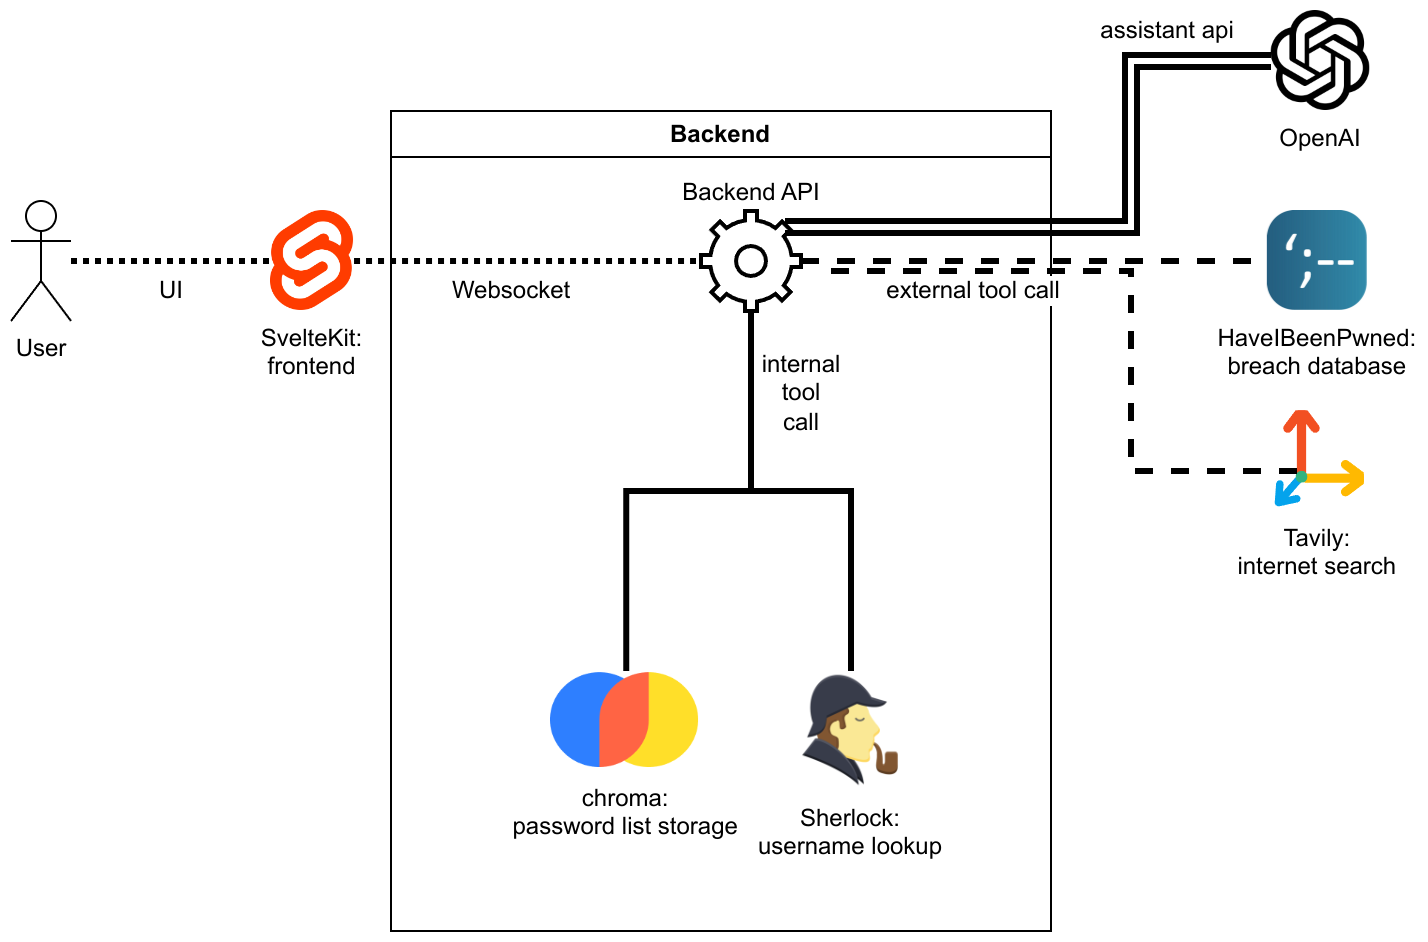
\includegraphics[width=14cm]{Structure200.png}
	\caption{Structure of the application}
	\label{fig:structure}
\end{figure} 

The user interacts with the frontend. \\
The frontend then sends a request to the central backend API, which calls all the other APIs and tools.

\subsection{Tools and APIs}
We have decided to use a combination of different APIs and tools, the following chapters will explain the tools and their integration into the project.

\subsubsection{chroma}
we use chroma \footnote{\url{https://www.trychroma.com/}}, a verctor based database to store list of leaked passwords. These lists were obtained from the GitHub repository \hyperlink{https://github.com/00xBAD/kali-wordlists}{00xBAD/kali-wordlists} which contains a number of different lists. We decided to use the following wordlists, which contain a mix of different passwords:
\begin{enumerate}
	\item wifite
	\item vnc\_passwords
	\item unix\_passwords
	\item sqlmap
	\item password
	\item keyboard-patterns
	\item fasttrack
	\item default\_pass\_for\_services\_unhash
	\item common
	\item adobe\_top100\_pass
\end{enumerate}
More wordlists could be added at any time and will be loaded when a new thread is created.

\subsubsection{Sherlock}
Sherlock \footnote{\url{https://github.com/sherlock-project/sherlock}} is a command line interface tool which searches for usernames across 400 social media sites and networks.
\\ \\
The tool has been modified to be used as an internal tool, without the need to call it via a new process.
\\ \\
By utilizing Sherlock, users can scan for usernames across numerous social networks, identify old accounts, detect impersonation attempts, and take appropriate action.

\subsubsection{HaveIBeenPwned}
HaveIBeenPwned \footnote{\url{https://haveibeenpwned.com/}} is an online tool which searches for a given email in data breaches and informs the user of those breaches.
\\ \\
''A data breach is any security incident in which unauthorized parties access sensitive or confidential information, including personal data (Social Security numbers, bank account numbers, healthcare data) and corporate data (customer records, intellectual property, financial information).''\cite{what-is-data-breach}
\\ \\
We use the API provided by HaveIBeenPwned to inform the user about breaches.

\subsubsection{tavily}
We also use tavily \footnote{\url{https://tavily.com/}}, an API to search the internet, which is optimized for LLMs.
\\ \\
We use Tavily to look up new and up-to-date information on security and privacy-related topics.

\subsection{Challenges}
The following chapters show the different challenges we faced during the development and the solutions we implemented to overcome the challenges.

\subsubsection{Frontend}
One of the first challenges was the frontend. We had specific requirements and ideas to show the user the output of the application, to summarize it, and to get the user input in an intuitive way.
\\ \\
The goal was to show all the output on the left and have a chat on the right side, as shown in the following image:
\begin{figure}[H]
	\centering
	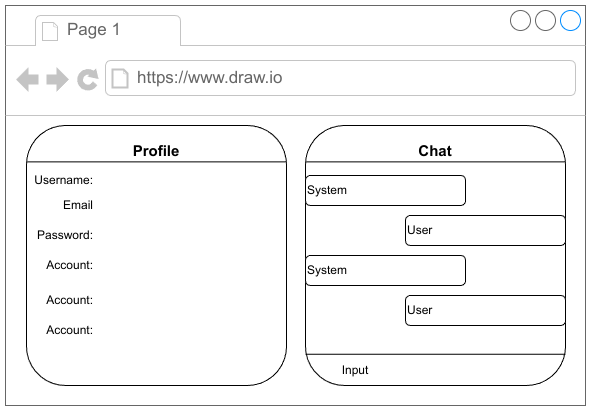
\includegraphics[width=10cm]{Frontend-draft.png}
	\caption{Draft of the frontend}
	\label{fig:draft-frontend}
\end{figure} 
None of the publicly available frontend libraries provided a solution to our requirements. To resolve this we created our own frontend using SvelteKit.

\subsubsection{Frontend - Connection to the Backend}
By building our own frontend, we faced the challenge of transporting information from the frontend to the backend, and back again. The first attempt, using a simple API on both sides failed.
\\ \\
We then transitioned to websockets, which allow the streaming of data to a listener. By doing so the frontend can send messages whenever and then listens to the response of the backend. This solved timeouts and other issues.

\subsubsection{Finding Sources and APIs}
Another challenge was the sourcing of information and tools to use in our application. While APIs and sources exist on the internet, most of them were behind a paywall or only available as tools to run locally.
\\ \\
We fixed the issues of local tooling by writing custom APIs for those tools, like spiderfoot \footnote{\url{https://github.com/smicallef/spiderfoot}}. Those APIs are being called by our backend.
\\ \\
In the end we ended up paying for the most important and useful APIs, like HaveIBeenPwned  \footnote{\url{https://haveibeenpwned.com/}}.

\subsubsection{Integrating Sherlock}
Since Sherlock is designed as a command-line interface tool, integrating it into the application was challenging.
\\ \\
We had to modify its code, removing most parts that control input and output, including argument parsing and scanning.

\subsubsection{Giving the User a Score}
We aimed to provide users with a score based on their level of privacy or lack thereof.  However, coming up with a formula was not possible.
\\ \\
One issue was the "living off the land" concept we used, relying solely on the data the user provided. We had no way of knowing if the user had given us all relevant information.
\\ \\
Another challenge was determining the weight of the issues found by the tools. For instance, is a breach worse than a leaked password?
\\ \\
Additionally, we had no way of knowing if the user had already resolved an issue. For example, there was no way to verify if a user had changed a leaked password.
\\ \\
Given these issues, providing the user with a score would create a false sense of security.

\section{Using Project AOPSE}
The project can be run locally. The setup is described in the readme.md in the GitHub repository of the project on \hyperlink{https://github.com/c-jaenicke/project-aopse}{c-jaenicke/project-aopse}.
\\ \\
The following prompts, or prompts similar to these, will execute a specific tool:
\begin{itemize}
	\item \lstinline[breaklines]|check the username <username>|: will start a search for the username on different social media networks
	\item \lstinline[breaklines]|check the password <password>|: will check if the password is present in one of the wordlists and give advice
	\item \lstinline[breaklines]|has the email <email address> been breached|: will check if the given email address has been found in any breaches
	\item \lstinline[breaklines]|is there any new information on <topic>|: will check for new information or news on the topic
\end{itemize}
In addition to those prompts, any prompt will lead to a result based on the previous messages and context provided.

\section{Future Plans}
As this is the first version, we have exciting plants for future developments.
\\ \\
This includes the development of a custom AI-model, as to not rely on OpenAI. 
Improving the performance of the backend. Possibly a full rewrite in a more advanced and safe language, like Rust \footnote{\url{https://www.rust-lang.org/}}. 
While also improving the security further. 
Implementing more tools and sources of information. 
And adding customizable search parameters.

% Referenzen bitte in references.bib einfügen
\newpage

\bibliographystyle{ieeetr}
\bibliography{references}

\end{document}
